% 
%  chapter3.tex
%  ISELthesis
%  
%  Created by Matilde Pós-de-Mina Pato on 2012/10/09.
%
\chapter{Trabalho realizado e por realizar}
\label{capitulo:trabalho-realizado-e-por-realizar}

Esta secção descreve o progresso atual do trabalho, bem como os objetivos principais. Para além disso é apresentada a análise do padrão dos dados e as funcionalidades previstas do sistema. O trabalho futuro incluirá o desenvolvimento das soluções propostas, com a implementação dos algoritmos e a realização de testes para avaliar a eficácia e a viabilidade do sistema.

Na Secção~\ref{capitulo3:Diagrama-blocos}, é apresentado o diagrama de blocos do sistema a desenvolver. Este diagrama proporciona uma estrutura organizada ao projeto e oferece uma visão abrangente dos seus principais componentes.

Na Secção~\ref{capitulo3:Requisitos-funcionais-nao-funcionais}, são definidos os requisitos funcionais e não funcionais do sistema. A especificação destes requisitos permite clarificar as funcionalidades previstas, bem como estabelecer a respetiva prioridade de implementação.

A Secção~\ref{capitulo3:Padrao-itc2019} apresenta uma análise detalhada do padrão adotado no projeto. Adicionalmente, são discutidas as adaptações realizadas para alinhar o padrão com os requisitos específicos do sistema em desenvolvimento.

Na Secção~\ref{capitulo3:Casos-util}, são descritos os casos de utilização, que representam os diferentes cenários de interação entre o utilizador e o sistema. Estes casos são fundamentais para compreender o funcionamento da aplicação, ajudando a validar os requisitos definidos e a garantir que todas as funcionalidades essenciais são consideradas no desenvolvimento.

A Secção~\ref{capitulo3:Restricoes} aborda as restrições consideradas na geração dos horários. A definição destas restrições é crucial, uma vez que influenciam diretamente a qualidade e a viabilidade dos horários produzidos.

A Secção~\ref{capitulo3:Diagrama-gantt} apresenta o diagrama de Gantt do projeto, onde é detalhado o planeamento das tarefas a realizar, incluindo a respetiva duração e dependências entre atividades.

Por fim, na Secção~\ref{capitulo3:Tarefas-principais-secundarias}, são delineadas as tarefas principais e secundárias na implementação do sistema, justificando a distinção entre ambas. Além disso, é avaliada a complexidade das tarefas e identificados os aspetos mais desafiantes do projeto.

\section{Diagrama de blocos do sistema}
\label{capitulo3:Diagrama-blocos}

Para garantir uma organização sólida, é essencial criar um diagrama de blocos que represente a estrutura geral do sistema a desenvolver. Esse diagrama fornecerá uma visão abrangente dos principais componentes, facilitando a compreensão das relações e dependências desde o início do desenvolvimento.

A Figura~\ref{fig:diagrama-blocos} apresenta o diagrama de blocos do sistema a desenvolver.

\begin{figure}[htb]
    \centering
    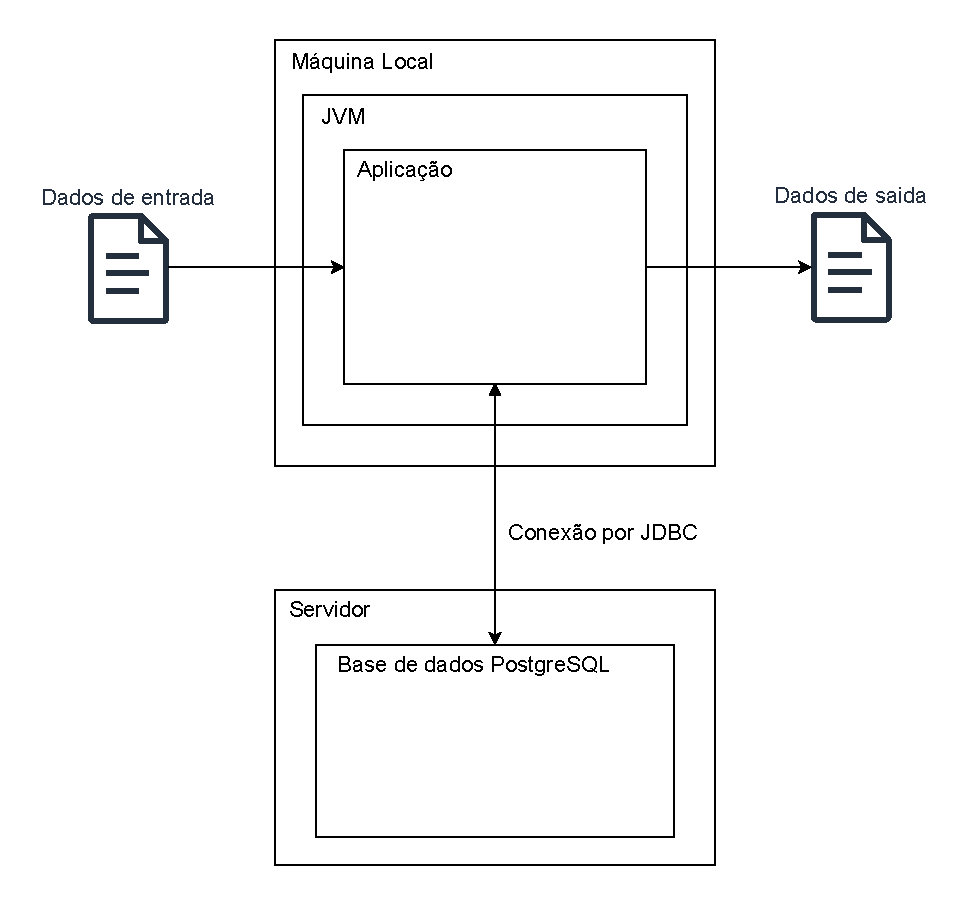
\includegraphics[width=.85\linewidth]{diagrama-blocos}
    \caption{Diagrama de blocos do sistema.}
    \label{fig:diagrama-blocos}
\end{figure}

A linguagem de programação escolhida para o desenvolvimento do sistema será Java, devido à sua capacidade de criar aplicações independentes do sistema operativo, ao vasto suporte proporcionado por bibliotecas e à sua eficiência na construção de soluções rápidas e robustas.

A base de dados adotada será relacional, o que facilita a estruturação e normalização dos dados armazenados. Dado que os dados a serem armazenados estão inter-relacionados, a utilização de uma base de dados relacional permitirá uma gestão mais eficaz dessas relações.

O sistema de gestão de base de dados selecionado é o PostgreSQL, reconhecido pela sua robustez e capacidade de lidar com grandes volumes de dados. À medida que o sistema crescer, a base de dados também se expandirá, sendo que o PostgreSQL assegura uma gestão eficaz mesmo em cenários de maior escala.

Para a comunicação entre o sistema de geração de horários e o servidor PostgreSQL, será utilizado o \gls{jdbc}, garantindo uma integração eficiente e fiável entre a aplicação e a base de dados. O \gls{jdbc} permite escrever diretamente as consultas \gls{sql} sem aumentar a complexidade do sistema.

\newpage % Correção temporária, serve para corrigir a colocação de tabelas e imagens

\section{Requisitos funcionais e não funcionais}
\label{capitulo3:Requisitos-funcionais-nao-funcionais}

Cada requisito é classificado como ''Obrigatório'' ou ''Opcional'', de acordo com a sua prioridade de implementação.

\begin{compactitem}
    \item Obrigatório: Indica que o requisito deve ser implementado dentro do prazo estipulado;
    \item Opcional: Refere-se a requisitos cuja implementação está condicionada à disponibilidade de tempo. Caso não seja viável dentro do cronograma, esses requisitos poderão ser descartados sem comprometer a funcionalidade essencial do sistema.
\end{compactitem}

A Tabela~\ref{tabela:requisitos-funcionais} apresenta os requisitos funcionais do sistema. Os requisitos funcionais descrevem funcionalidades, comportamentos e operações específicas que o sistema deve realizar para atender às necessidades do utilizador. A sua classificação depende do impacto na concretização de um sistema funcional e eficaz. Se um requisito for essencial para o correto funcionamento do sistema, é classificado como ''Obrigatório'', caso contrário, é considerado ''Opcional''.

{
\setlength{\tabcolsep}{.8em}
\begin{table}[H]
    \centering
    \caption{Requisitos funcionais.}
    \label{tabela:requisitos-funcionais}
    \begin{tabular}{c p{0.6\linewidth} c}
        \toprule
        \textbf{Referência} & \multicolumn{1}{c}{\textbf{Descrição}} & \textbf{Classificação} \\ \midrule
        RF001      & Manipular os horários criados através da interface gráfica                             & Obrigatório   \\ \midrule
        RF002      & Persistência de dados, de entrada e saída, através de uma base de dados                & Obrigatório   \\ \midrule
        RF003      & Horários modificados devem ser guardados em ficheiros distintos dos originais          & Obrigatório   \\ \midrule
        RF004      & A criação de horários deve permitir criar manchas de disponibilidade institucionais    & Obrigatório   \\ \midrule
        RF005      & Apresentação de erros ao utilizador caso a aplicação falhe nalguma operação            & Obrigatório   \\ \midrule
        RF006      & Na interface gráfica devem ser apresentados os dados presentes na base de dados        & Obrigatório   \\ \midrule
        RF007      & Através da interface gráfica deve ser possível alterar os dados na base de dados       & Obrigatório   \\ \midrule
        RF008      & Congelamento de salas e/ou professores no momento de geração dos horários              & Opcional      \\ \midrule
        RF009      & Alteração das manchas através da interface gráfica                                     & Opcional      \\ \midrule
        RF010      & Através da interface gráfica definir períodos para as aulas partilhadas                & Opcional      \\ \bottomrule
    \end{tabular}
\end{table}
}

\newpage % Correção temporária, serve para corrigir a colocação de tabelas e imagens

Na Tabela~\ref{tabela:requisitos-nao-funcionais} são listados os requisitos não funcionais do sistema. Os requisitos não funcionais definem como o sistema deve funcionar. Estes descrevem restrições, padrões de qualidade e atributos que influenciam o seu desempenho. A sua classificação segue a lógica dos requisitos funcionais.

{
\setlength{\tabcolsep}{.8em}
\begin{table}[htbp]
    \centering
    \caption{Requisitos não funcionais.}
    \label{tabela:requisitos-nao-funcionais}
    \begin{tabular}{c p{0.6\linewidth} c}
        \toprule
        \textbf{Referência} & \multicolumn{1}{c}{\textbf{Descrição}} & \textbf{Classificação} \\ \midrule
        RNF001     & A interface gráfica deve ser intuitiva e permitir a edição manual dos horários gerados   & Obrigatório   \\ \midrule
        RNF002     & Existência de \textit{feedback} visual, como barras de progresso, durante a geração dos horários & Obrigatório   \\ \midrule
        RNF003 &
        Exportação de dados nos formatos \gls{xml} e \gls{csv}, sendo os formatos \gls{png} e \gls{pdf} exclusivos para os horários &
        Obrigatório \\ \midrule
        RNF004     & Criação de \textit{logs} detalhados do funcionamento do sistema                          & Opcional      \\ \bottomrule
    \end{tabular}
\end{table}
}

\section{Estrutura do padrão da ITC 2019}
\label{capitulo3:Padrao-itc2019}

A definição e representação dos horários serão feitas com base no padrão introduzido pela \gls{itc}~2019. Para que se possa concretizar a definição dos horários é necessário primeiro compreender o padrão.

Na \gls{itc}~2019 são apresentados conjuntos de instâncias que podem ser utilizadas para testar o funcionamento do sistema. Os dados encontram-se no formato \gls{xml} e contêm \textit{tags} que permitem definir múltiplas informações, tais como horários de funcionamento, salas, disciplinas e estudantes.

Os exemplos apresentados encontram-se diretamente na página da competição \cite{itc2019-Website}, ou nas instâncias lá disponibilizadas.

\subsection{Horários de funcionamento}

A \textit{tag} principal apresenta o número de dias por semana, a quantidade de \textit{slots} diários e a duração do semestre, em semanas, que o horário deve conter.

Entende-se como \textit{slot} um bloco ao qual se pode atribuir uma aula. Quanto mais \textit{slots} por dia maior é a granularidade no momento de atribuição das aulas aos vários períodos de tempo disponíveis. Para ajudar na compreensão encontra-se na Listagem~\ref{listagem:exemplo-duracao-semestre} um exemplo.

\begin{minipage}[c]{\linewidth}
\begin{lstlisting}[caption={Exemplo da definição da duração do semestre.}, label={listagem:exemplo-duracao-semestre}]
<problem name="unique-instance-name" nrDays="7" nrWeeks="13" slotsPerDay="288">
\end{lstlisting}
\end{minipage}

Neste caso, cada semana tem 7 dias e o semestre letivo tem duração de 13 semanas. Para obter a duração de cada \textit{slot} é necessário dividir o número de minutos, num único dia, pelo número de \textit{slots} totais, ou seja, $24*60/288 = 5$. Verifica-se que cada \textit{slot} tem a duração de 5 minutos.

\subsection{Aulas}

Para definir os horários das aulas serão utilizados os \textit{slots} definidos anteriormente. Na Listagem~\ref{listagem:exemplo-aula} encontra-se um exemplo da definição de uma aula. A definição de cada aula deve ser efetuada no contexto da definição da respetiva disciplina, mas neste caso simplificado, apenas será mostrada a definição da aula.

\begin{minipage}[c]{\linewidth}
\begin{lstlisting}[caption={Exemplo da definição de uma aula.}, label={listagem:exemplo-aula}]
<class id="1" limit="22">
    <room id="10" penalty="0"/>
    <room id="11" penalty="0"/>
    <room id="12" penalty="0"/>
    <time days="0100000" start="90" length="22" weeks="111111111111111" penalty="0"/>
    <time days="0010000" start="90" length="22" weeks="111111111111111" penalty="0"/>
    <time days="0001000" start="90" length="22" weeks="111111111111111" penalty="0"/>
</class>
\end{lstlisting}
\end{minipage}

Na \textit{tag class} é definido o identificador da aula e a quantidade limite de estudantes que podem frequentar a aula. O limite apresentado apenas faz sentido na formulação \gls{pe-ctt}, pois desta forma tem-se acesso à quantidade de estudantes que devem frequentar a disciplina em causa.

A definição dos dias em que a aula fica agendada encontra-se num formato binário e inicia-se na segunda-feira. De acordo com o exemplo, a aula deve ocorrer na segunda-feira, quarta-feira ou sexta-feira.

Para calcular a hora de início da aula, é necessário multiplicar a duração de cada \textit{slot} pelo \textit{offset} apresentado no \textit{start} e de seguida converter para horas, ou seja, $início = 5*90/60 = 7,5$, de acordo com o resultado, a aula deve ter início às 7:30 da manhã.

A duração da aula deve ser de 1 hora e 50 minutos e pode ser calculada da mesma forma que o início da aula, ou seja, $duração = 5*22 = 110$. Verificando agora as semanas em que a aula deve ser agendada, verifica-se que esta deve estar agendada para todas as semanas. Por fim, é definida uma penalização caso o horário não siga a definição na sua totalidade.

\subsection{Salas}

No momento de definição de salas é possível definir o seu identificador, a sua lotação máxima, a distância das outras salas e períodos de indisponibilidade. Apresenta-se um exemplo na Listagem~\ref{listagem:exemplo-salas}.

\begin{minipage}[c]{\linewidth}
\begin{lstlisting}[caption={Exemplo da definição das salas.}, label={listagem:exemplo-salas}]
<rooms>
    <room id="1" capacity="61">
        <travel room="2" value="12"/>
        <unavailable days="0010000" start="222" length="36" weeks="111111111111111"/>
    </room>
    <room id="2" capacity="36">
        <travel room="4" value="12"/>
        <travel room="5" value="12"/>
    </room>
</rooms>
\end{lstlisting}
\end{minipage}

No exemplo apresentado são definidas duas salas. A sala 1 tem lotação de 61 estudantes e a sala 2 tem lotação de 36 estudantes. Para cada sala, são apresentadas as distâncias às outras salas. A definição das distâncias é importante no caso de duas aulas consecutivas, por exemplo uma aula na sala 1 e de seguida uma aula na sala 2, pois os estudantes têm de fazer o percurso entre ambas as salas. É um atributo relevante para otimizar a seleção das salas, caso se encontrem muito afastadas.

Os períodos de indisponibilidade são definidos de forma muito semelhante aos horários de funcionamento das aulas.

A lotação das salas não terá importância neste projeto pois os horários são criados antes das inscrições dos estudantes, o que impossibilita a utilização desta restrição.

\subsection{Disciplinas}

No padrão apresentado, a palavra \textit{course} refere-se a uma disciplina. A definição das disciplinas podem ter uma hierarquia complexa de aulas. Para que a hierarquia possa ser representada, o padrão permite a declaração das mesmas através da criação de configurações e subpartes. Cada disciplina pode ter várias configurações e cada configuração pode ter várias subpartes, sendo que apenas as subpartes devem conter as aulas.

Cada aluno deve assistir a uma das aulas presentes em cada subparte numa única configuração. Cada aula pode ainda ter um progenitor, o que indica que para assistir a dita aula é necessário assistir também à aula progenitora.

É apresentado um exemplo da definição de uma disciplina na Listagem~\ref{listagem:exemplo-disciplinas}.

\begin{minipage}[c]{\linewidth}
    \begin{lstlisting}[caption={Exemplo da definição de uma disciplina.}, label={listagem:exemplo-disciplinas}]
<course id="ME 263">
    <config id="1">
        <subpart id="1_Lecture">
            <class id="Lec1" limit="100"/>
            <class id="Lec2" limit="100"/>
        </subpart>
        <subpart id="2_Recitation">
            <class id="Rec1" limit="50"/>
            <class id="Rec2" limit="50"/>
            <class id="Rec3" limit="50"/>
            <class id="Rec4" limit="50"/>
        </subpart>
    </config>
    <config id="2">
        <subpart id="3_Lecture">
            <class id="Lec3" limit="100"/>
            <class id="Lec4" limit="100"/>
        </subpart>
        <subpart id="4_Recitation">
            <class id="Rec5" parent="Lec3" limit="50"/>
            <class id="Rec6" parent="Lec3" limit="50"/>
            <class id="Rec7" parent="Lec4" limit="50"/>
            <class id="Rec8" parent="Lec4" limit="50"/>
        </subpart>
        <subpart id="5_Laboratory">
            <class id="Lab1" parent="Rec5" limit="50"/>
            <class id="Lab2" parent="Rec6" limit="50"/>
            <class id="Lab3" parent="Rec7" limit="50"/>
            <class id="Lab4" parent="Rec8" limit="50"/>
        </subpart>
    </config>
</course>
    \end{lstlisting}
\end{minipage}

%TODO: por concluir

\subsection{Estudantes}

A definição dos estudantes consiste na atribuição de um identificador único, como o número mecanográfico do aluno, e na especificação das disciplinas a que se inscreveu. Na Listagem~\ref{listagem:exemplo-estudantes}, é apresentado um exemplo para ilustrar a definição dos estudantes.

\begin{minipage}[c]{\linewidth}
\begin{lstlisting}[caption={Exemplo da definição dos estudantes.}, label={listagem:exemplo-estudantes}]
<students>
    <student id="1">
        <course id="4"/>
    </student>
</students>
\end{lstlisting}
\end{minipage}

Esta funcionalidade não será utilizada neste projeto devido ao \gls{isel} não permitir as pré-inscrições dos estudantes.

\subsection{Restrições}

No padrão podem ser definidas várias restrições, apresentadas na Figura~\ref{fig:restricoes-itc2019}.

\begin{figure}[ht]
    \centering
    \includegraphics[width=.75\linewidth]{restricoes-itc2019}
    \caption{Restrições suportadas no padrão da ITC 2019 (adaptado de \cite{itc2019-Website}).}
    \label{fig:restricoes-itc2019}
\end{figure}

Em seguida, são apresentadas descrições das várias restrições, adaptadas de \cite{itc2019-Website}.

\begin{compactitem}
    \item SameStart - Todas as aulas devem começar à mesma hora;

    \item SameTime - Todas as aulas devem ocorrer nos mesmos horários do dia exigidos pela aula mais longa do conjunto;

    \item DifferentTime - Todas as aulas devem estar não sobrepostas;

    \item SameDays - Todas as aulas devem ocorrer nos mesmos dias da semana. Caso uma das aulas seja lecionada num número reduzido de dias em relação às outras, esta deve ser lecionada num subconjunto dos dias utilizados pela aula com maior número de dias;

    \item DifferentDays - Todas as aulas devem ser lecionadas em dias da semana diferentes;

    \item SameWeeks - Todas as aulas devem ser lecionadas nas mesmas semanas. Caso uma das aulas seja lecionada num número reduzido de semanas em relação às outras, esta deve ser lecionada num subconjunto das semanas utilizadas pela aula com maior número de semanas;

    \item DifferentWeeks - Todas as aulas devem ser lecionadas em semanas diferentes;

    \item SameRoom - Todas as aulas devem ser lecionadas na mesma sala;

    \item DifferentRoom - Todas as aulas devem ser lecionadas em salas diferentes;

    \item Overlap - Quaisquer duas aulas nesta restrição devem ter alguma sobreposição no tempo. Implica sobreposição no período do dia, nos dias da semana e semanas;

    \item NotOverlap - As duas aulas não se podem sobrepor no tempo;

    \item SameAttendees - Todas as aulas devem ocorrer em horários e locais tais que alguém que deva comparecer seja capaz de assistir a todas as aulas;

    \item Precedence - Estabelece uma ordem que exige que a primeira reunião da primeira aula listada ocorra na sua totalidade antes da primeira reunião da aula que se segue na ordem, repetindo a lógica para as restantes aulas;

    \item WorkDay(S) - Previne ou penaliza quando o número de períodos entre o início da primeira aula e o fim da última aula excede o número de períodos ''S'' definido na restrição;

    \item MinGap(G) - Os horários atribuídos a quaisquer duas aulas que sejam colocadas no mesmo dia devem permitir pelo menos ''G'' \textit{slots} entre o final da aula anterior e o início da aula posterior;

    \item MaxDays(D) - As aulas não podem ser distribuídas por mais de ''D'' dias diferentes da semana independentemente de estarem em semanas distintas do período letivo.

    \item MaxDayLoad(S) - Limita a quantidade total de tempo atribuído ao conjunto de aulas a não mais do que ''S'' intervalos de tempo por dia, durante todo o semestre;

    \item MaxBreaks(R,S) - Limita o número de intervalos entre aulas durante o dia que excedem ''S'' períodos de tempo, garantindo que não sejam superiores a ''R'' por dia;

    \item MaxBlock(M,S) - Limita a quantidade de tempo (medida em ''M'' \textit{slots}) durante a qual um conjunto de aulas pode ser agendado de forma consecutiva, sendo que cada uma delas está separada por no máximo ''S'' \textit{slots}.
\end{compactitem}

Sabendo as restrições suportadas pelo padrão, é apresentado na Listagem~\ref{listagem:exemplo-restricoes} um exemplo da definição das restrições. Cada restrição pode ser rígida ou flexível, sendo as suas definições `required="true"'' e `penalty="4"'' (ou outro valor) respetivamente.

\begin{minipage}[c]{\linewidth}
\begin{lstlisting}[caption={Exemplo da definição das restrições.}, label={listagem:exemplo-restricoes}]
<distributions>
    <distribution type="SameAttendees" required="true">
        <class id="140"/>
        <class id="155"/>
        <class id="156"/>
    </distribution>
    <distribution type="NotOverlap" required="true">
        <class id="91"/>
        <class id="92"/>
        <class id="93"/>
        <class id="94"/>
    </distribution>
    <distribution type="SameRoom" penalty="4">
        <class id="81"/>
        <class id="82"/>
    </distribution>
</distributions>
\end{lstlisting}
\end{minipage}

No exemplo são apresentadas três restrições diferentes. Dentro de cada bloco, são colocados os identificadores das aulas que possuem tal restrição.

\subsection{Modificações propostas}

Para a criação dos horários é necessário incluir os dados relativos aos professores que irão lecionar as aulas agendadas. Para permitir a inclusão dessa informação será necessário incluir esses dados no padrão. Na Listagem~\ref{listagem:padrao-exemplo-professores}, encontra-se um exemplo da definição dos dados relativos aos professores.

\begin{minipage}[c]{\linewidth}
\begin{lstlisting}[caption={Exemplo da informação relacionada com os professores.}, label={listagem:padrao-exemplo-professores}]
<teachers>
    <teacher id="1" name="Rui Antunes">
        <class id="1"/>
        <class id="2"/>
        <unavailable days="0010000" start="222" length="36" weeks="111111111111111"/>
    </teacher>
    <teacher id="2" name="João Rodrigues">
        <class id="3"/>
        <class id="4"/>
    </teacher>
</teachers>
\end{lstlisting}
\end{minipage}

Cada professor pode lecionar várias disciplinas e também pode ter manchas de indisponibilidade. Cada professor é identificado pelo seu número mecanográfico, atribuído pela instituição, e pelo seu nome. A definição das manchas de indisponibilidade segue o formato estabelecido na definição das salas.

\section{Casos de utilização}
\label{capitulo3:Casos-util}

Os casos de utilização descrevem, de forma precisa, as interações entre o utilizador e o sistema, identificando funcionalidades específicas e os objetivos a serem alcançados. Em todos os casos de utilização apresentados, o ator principal é o utilizador da aplicação, que interage com o sistema para realizar tarefas como a inserção de dados, criação de horários e visualização de informações. Cada caso de utilização descreve os passos sequenciais que o utilizador deve seguir para completar uma tarefa específica.

\subsection*{Caso de Utilização 1 - Inserção de dados através de ficheiro}
Leitura de um ficheiro, organizado de acordo com o padrão da \gls{itc}~2019, e armazenamento dos dados numa base de dados.

Cenário principal:

\begin{compactenum}
    \item O caso de utilização inicia-se quando o utilizador pressiona o botão de inserção de dados através de ficheiro.
    \item O utilizador escolhe o ficheiro que deve ser lido por parte da aplicação. \label{casos-util-1:escolha-ficheiro}
    \item A aplicação processa os dados. \label{casos-util-1:processar-dados}
    \item A aplicação armazena os dados na base de dados. \label{casos-util-1:armazenar-dados}
    \item O caso de utilização termina.
\end{compactenum}

Cenário alternativo 1:

\begin{compactenum}
    \item No passo~\ref{casos-util-1:escolha-ficheiro}, o utilizador cancela a escolha do ficheiro.
    \item O caso de utilização termina.
\end{compactenum}

Cenário alternativo 2:

\begin{compactenum}
    \item No passo~\ref{casos-util-1:processar-dados}, o ficheiro escolhido não segue o padrão da \gls{itc}~2019.
    \item Apresentação de uma mensagem de erro ao utilizador.
    \item O caso de utilização termina.
\end{compactenum}

Cenário alternativo 3:

\begin{compactenum}
    \item No passo~\ref{casos-util-1:armazenar-dados}, ocorreu um erro no armazenamento dos dados, o qual não pôde ser resolvido.
    \item Apresentação de uma mensagem de erro ao utilizador.
    \item O caso de utilização termina.
\end{compactenum}

\subsection*{Caso de Utilização 2 - Inserção de dados manual}
Inserção de dados relativos a salas, professores ou disciplinas manualmente.

Cenário principal:

\begin{compactenum}
    \item O caso de utilização inicia-se quando o utilizador pressiona o botão de inserção de dados manual (este pode ser relativo a salas, professores ou disciplinas).
    \item O utilizador preenche a informação relativa à categoria escolhida. \label{casos-util-2:preench-dados}
    \item A aplicação processa os dados. \label{casos-util-2:processar-dados}
    \item A aplicação armazena os dados na base de dados. \label{casos-util-2:armazenar-dados}
    \item O caso de utilização termina.
\end{compactenum}

Cenário alternativo 1:

\begin{compactenum}
    \item No passo~\ref{casos-util-2:preench-dados}, o utilizador pressiona o botão para cancelar a inserção de dados.
    \item O caso de utilização termina.
\end{compactenum}

Cenário alternativo 2:

\begin{compactenum}
    \item No passo~\ref{casos-util-2:processar-dados}, os dados introduzidos não estão de acordo com o padrão.
    \item Apresentação de uma mensagem de erro ao utilizador.
    \item O caso de utilização termina.
\end{compactenum}

Cenário alternativo 3:

\begin{compactenum}
    \item No passo~\ref{casos-util-2:armazenar-dados}, ocorreu um erro no armazenamento dos dados, o qual não pôde ser resolvido.
    \item Apresentação de uma mensagem de erro ao utilizador.
    \item O caso de utilização termina.
\end{compactenum}

\subsection*{Caso de Utilização 3 - Criação de horários}
Após o clique no botão de criação de horários, o programa deve gerar os horários, conforme a configuração especificada, e apresentar os horários gerados na interface gráfica.

Pré-condições: Existência de dados armazenados na base de dados.

Cenário principal:

\begin{compactenum}
    \item O caso de utilização inicia-se quando o utilizador pressiona o botão de criação de horários.
    \item A aplicação processa os dados armazenados e cria os horários pedidos. \label{casos-util-3:gerar-horarios}
    \item São apresentados os horários gerados através da interface gráfica.
    \item O caso de utilização termina.
\end{compactenum}

Cenário alternativo 1:

\begin{compactenum}
    \item No passo~\ref{casos-util-3:gerar-horarios} não foi possível gerar os horários devido às restrições.
    \item Apresentação de uma mensagem de erro ao utilizador, detalhando as restrições que causaram a falha.
    \item O caso de utilização termina.
\end{compactenum}

\subsection*{Caso de Utilização 4 - Visualização de horário criado}
Após selecionado um dos horários gerados, de uma lista de horários, apresentados na interface gráfica, deve ser apresentado o horário de forma ampliada.

Pré-condições: Existência de horários gerados previamente.

Cenário principal:

\begin{compactenum}
    \item O caso de utilização inicia-se quando o utilizador seleciona um horário a partir de uma lista de horários gerados pela aplicação.
    \item A aplicação apresenta o horário de forma ampliada ao utilizador.
    \item O caso de utilização termina.
\end{compactenum}

\subsection*{Caso de Utilização 5 - Modificação de horário criado}
Após a seleção de um dos horários gerados de uma lista apresentada na interface gráfica, este deverá ser exibido, permitindo a sua modificação.

Pré-condições: Existência de horários gerados previamente.

Cenário principal:

\begin{compactenum}
    \item O caso de utilização tem início quando o utilizador seleciona um horário de uma lista de horários gerados pela aplicação.
    \item A aplicação apresenta o horário de forma ampliada ao utilizador.
    \item O utilizador modifica o horário ao mover as atribuições das aulas.
    \item O utilizador confirma as modificações através de um clique no botão de confirmação. \label{casos-util-5:confirmar-alteracoes}
    \item A aplicação armazena as alterações num novo horário de modo a não se perder o horário original.
    \item O caso de utilização termina.
\end{compactenum}

Cenário alternativo 1:

\begin{compactenum}
    \item No passo~\ref{casos-util-5:confirmar-alteracoes} o utilizador pressiona o botão para cancelar as alterações efetuadas ao horário.
    \item O caso de utilização termina.
\end{compactenum}

\subsection*{Caso de Utilização 6 - Exportação dos horários criados}
São exportados os horários selecionados no formato escolhido para a localização que o utilizador especificou.

Pré-condições: Existência de horários gerados previamente.

Cenário principal:

\begin{compactenum}
    \item O caso de utilização inicia-se quando o utilizador seleciona a opção de exportar horários.
    \item O utilizador seleciona o formato no qual o horário deve ser exportado, sendo os seguintes formatos suportados \gls{xml}, \gls{pdf}, \gls{csv} e \gls{png}.
    \item O utilizador deve especificar o local para o qual os horários serão exportados.
    \item A aplicação efetua a exportação do horário.
    \item O caso de utilização termina.
\end{compactenum}

\section{Restrições para a criação dos horários}
\label{capitulo3:Restricoes}

Nesta secção são estabelecidas as restrições a considerar na elaboração dos horários. As restrições rígidas correspondem a condições indispensáveis, cuja violação tornaria o horário inviável. Já as restrições flexíveis referem-se a situações que, idealmente, devem ser evitadas, mas que podem ser aceites caso não existam alternativas viáveis.

\subsection{Restrições rígidas}

As restrições rígidas incluem sobreposições de aulas, conflitos de salas e indisponibilidades dos professores. O incumprimento de qualquer uma destas restrições inviabiliza a utilização do horário gerado.

\begin{compactenum}
    \item Ocupação de salas: Aulas agendadas no mesmo período devem ser concretizadas em salas distintas;
    \item Conflitos de disciplinas obrigatórias: Não haver sobreposições entre disciplinas quando, pelo menos, uma delas for obrigatória;
    \item Indisponibilidade dos professores: Caso os professores apresentem períodos de indisponibilidade, não deverão ser agendadas aulas nesses períodos para esses docentes.
\end{compactenum}

\subsection{Restrições flexíveis}

As restrições flexíveis incluem redução do número de salas ocupadas e redução de intervalos entre aulas. Estas restrições pretendem aumentar a qualidade da solução final.

\begin{compactenum}
    \item Número de salas: O número de salas distintas utilizadas pela disciplina deve ser o menor possível;
    \item Intervalos entre aulas: Evitar a existência de blocos de tempo sem aulas entre aulas consecutivas.
\end{compactenum}

\subsection{Decisões tomadas}

\subsubsection{Definição dos cursos}

O curso na base de dados é denominado de \textit{program} para não colidir com as disciplinas. Para que os dados fornecidos pelo padrão fiquem ligados a um curso é utilizada a \textit{tag} \textit{name}. É apresentado um exemplo na Listagem~\ref{listagem:identificacao-curso}.

\begin{minipage}[c]{\linewidth}
\begin{lstlisting}[caption={Exemplo da identificação do curso.}, label={listagem:identificacao-curso}]
<problem name="MEIC" nrDays="7" slotsPerDay="288" nrWeeks="9">
\end{lstlisting}
\end{minipage}

%TODO: Falta explicar e terminar até próxima entrega

%\subsection{Método de busca}
%\label{capitulo3:Metodo-busca}

%\subsubsection{Espaço de busca}

%TODO: Por preencher

%\subsubsection{Relações de vizinhança}

%TODO: Por preencher

%\subsubsection{Função de custo}

%A função de custo consiste na soma das penalizações das restrições violadas. As penalizações das restrições devem-se encontrar nos dados fornecidos à aplicação.

%TODO: Por preencher

\section{Diagrama de Gantt - planeamento}
\label{capitulo3:Diagrama-gantt}

Na Figura~\ref{fig:diagrama-gantt}, apresenta-se o Diagrama de Gantt correspondente ao desenvolvimento deste projeto. Nele, estão detalhadas as principais fases, desde a análise inicial dos requisitos até à implementação e validação do sistema. Cada tarefa é representada por uma barra que indica o período de execução previsto, sendo que dentro de cada barra encontra-se o número de dias associado.

A utilização deste diagrama permite uma gestão eficiente do cronograma do projeto, facilitando o acompanhamento do progresso e a identificação de eventuais atrasos ou necessidade de ajustes. Além disso, proporciona uma visão estruturada do fluxo de trabalho auxiliando no cumprimento dos prazos estabelecidos.

\begin{figure}[H]
    \centering
    \begin{ganttchart}[
        x unit=0.05cm, % Ajusta o espaçamento horizontal
        y unit chart=0.7cm, % Ajusta o espaçamento vertical
        title height=1, % Retira a linha entre o ano e os meses
        y unit title=5mm, % Diminui o tamanho dos meses e ano
        title label font=\tiny\bfseries,
        group label font=\footnotesize\bfseries,
        bar label font=\scriptsize,
        group height=.5,
        group/.append style={draw=black, fill=teal},
        bar/.append style={draw=black, fill=cyan},
        time slot format=little-endian,
        progress label node/.append style={font=\tiny, text=black} % Formata a etiqueta de progresso
    ]{01.03.2025}{30.09.2025} % Define a escala do diagrama
      \gantttitlecalendar{year, month} \\

      \node (a) [anchor=east, yshift=-7pt] at (current bounding box.west){Meses:};
    
      \ganttgroup[progress=100, progress label text={213 dias}]{Escrita do TFM}{01.03.2025}{30.09.2025} \\

      \ganttgroup[progress=100, progress label text={159 dias}]{Implementação}{01.03.2025}{07.08.2025} \\
      \ganttbar[progress=100, progress label text={28 dias}]{Planeamento da Arquitetura}{01.03.2025}{29.03.2025} \\
      \ganttbar[progress=100, progress label text={21 dias}]{Interpretador ITC 2019}{29.03.2025}{19.04.2025} \\
      \ganttbar[progress=100, progress label text={21 dias}]{Base de Dados}{16.04.2025}{07.05.2025} \\
      \ganttbar[progress=100, progress label text={28 dias}]{Simulated Annealing}{04.05.2025}{01.06.2025} \\
      \ganttbar[progress=100, progress label text={41 dias}]{Interface Gráfica}{29.05.2025}{09.07.2025} \\
      \ganttbar[progress=100, progress label text={32 dias}]{Correção de erros}{06.07.2025}{07.08.2025} \\

      \ganttgroup[progress=100, progress label text={54 dias}]{Avaliação da Aplicação}{07.08.2025}{30.09.2025}
    
    \end{ganttchart}
    \caption{Diagrama de Gantt.}
    \label{fig:diagrama-gantt}
\end{figure}

\section{Tarefas principais e secundárias}
\label{capitulo3:Tarefas-principais-secundarias}

Identificam-se como tarefas principais do projeto:

\begin{compactitem}
    \item Implementação de um sistema de importação de dados \gls{xml} de acordo com o padrão da \gls{itc}~2019;
    \item Disponibilizar a importação manual dos dados;
    \item Apresentação de erros ao utilizador caso ocorra alguma falha no funcionamento do sistema;
    \item Apresentação de conflitos no caso de impossibilidade de criação de horários;
    \item Criação de interface gráfica simples e fácil de utilizar;
    \item Permitir ajustes manuais aos horários gerados;
    \item Implementação e otimização dos parâmetros do algoritmo \gls{sa};
    \item Implementação de base de dados para a persistência dos dados da aplicação;
    \item Apresentação de \textit{feedback} visual durante o processo de geração de horários.
\end{compactitem}

Identificam-se como tarefas secundárias do projeto:

\begin{compactitem}
    \item Definição de manchas de disponibilidade através da interface gráfica;
    \item Definição de períodos para aulas partilhadas através da interface gráfica;
    \item Criação de \textit{logs} detalhados do funcionamento do sistema;
    \item Congelamento de salas e/ou professores no momento de geração de horários.
\end{compactitem}

A distinção entre as tarefas principais e secundárias é determinada pelo objetivo principal de garantir uma aplicação funcional. O foco principal consiste em otimizar a geração dos horários e permitir que o utilizador interaja eficazmente com os dados armazenados na base de dados. As tarefas secundárias visam melhorar a interação do utilizador com a aplicação.

As tarefas previstas como mais simples e rápidas estão relacionadas com a implementação da base de dados e com o desenvolvimento do interpretador do padrão. Quando o planeamento é adequado, a implementação dessas funcionalidades torna-se uma tarefa relativamente simples.

Por outro lado, as tarefas mais complexas estão relacionadas com o desenvolvimento da interface gráfica e com a implementação e otimização do algoritmo \gls{sa}. A necessidade de que a interface gráfica seja intuitiva, eficiente e capaz de apresentar uma grande quantidade de informação com poucos cliques torna o seu desenvolvimento um processo desafiador. A implementação do \gls{sa} exige o seu funcionamento para múltiplos cronogramas de cursos em simultâneo, de forma a conciliar as restrições de cada um, de modo a ser possível gerar os horários para os diversos cursos. A otimização do \gls{sa} requer múltiplos testes e comparações de resultados, o que implica um investimento significativo de tempo, com o objetivo de encontrar parâmetros satisfatórios para o algoritmo.